\documentclass[aspectratio=169]{beamer}
\usetheme{metropolis}
\usepackage[T1]{fontenc}
\usepackage[utf8]{inputenc}
\usepackage{graphicx,relinput}
\relinput{.}{authors_cmd}
\DeclareUnicodeCharacter{2032}{\prime}
% Commands from `proofarticle.cls` (important to compile)
\newcommand{\Cfrw}{C_{\mathrm{fr}}^{(w)}}
\newcommand{\Thetaw}{\Theta_w}
\title{\texorpdfstring{Interdisciplinary Guide — T1$′$–T4 \& InterIA}{Interdisciplinary Guide — T1′–T4 \& InterIA}}
\author{\InterIAPDFAuthors}
\date{\today}
\begin{document}
\begin{frame}\titlepage\end{frame}
\begin{frame}{Reading routes}\small\section{Reading routes (by specialty)}
\textbf{NT.} T1$′$ → T2 → T3; T4 minimal. \\
\textbf{AO.} T2 → T1$′$ → T3; T4 as spectral reading. \\
\textbf{Signal.} Tapers, bandlimit; T2 as frame conditioning; T3 as matched-filter probe. \\
\textbf{Phys.} Rigidity (T2) + localized measurement (T3); HP compatible. \\
\textbf{Repro.} See InterIA (separate). \\
\textbf{Formal.} Lemmas: Schur/Gershgorin, PW density, Archimedean, absorption.
\end{frame}
\begin{frame}{Dictionary (condensed)}\scriptsize\section{Notations and preliminaries}
\begin{center}
\begin{tabular}{p{0.28\linewidth} p{0.64\linewidth}}
\hline
\textbf{NT} & \textbf{Cross reading} \\\hline
Band $[-A,A]$ & Bandwidth (signal) \\
Cos$^2$ taper & Apodization (plateau/transition) \\
$\Xi_A$ & Non-uniform sampling \\
$\log p/p^{k/2}$ & $p$–adic energy weighting \\
$\Cfrw\ge 1-\Thetaw$ & Frame conditioning (AO) \\
Wave–packet $\hat\phi_T$ & Matched filter (signal/phys) \\
Explicit formula & Source–spectrum coupling \\
\hline
\end{tabular}
\end{center}
\end{frame}
\begin{frame}{Storyboard T1$′$–T4}\small\section{\texorpdfstring{Storyboard T1$′$–T4}{Storyboard T1′–T4}}
T1$′$: set the arena (PW, explicit, Archimedean).\\
T2: gap via locality + weights. \\
T3: packet → contradiction if off-line zero. \\
T4: HP-compatible reading (no postulate).
\end{frame}
\begin{frame}{Bridges}\small\section{Bridges boxes}
\textbf{(AO)} $G^{(w)}$ Gram; $I+R$ with $\|R\|<1$ gives lower boundedness. \\
\textbf{(Signal)} Band $[-A,A]$, apodized taper, frame $\approx$ robust reconstruction. \\
\textbf{(Phys)} T2 = spectral rigidity; T3 = localized measurement. \\
\textbf{(Repro)} Interval certificates; proof does not depend on numerics.
\end{frame}
\begin{frame}{Micro-example T2}\small\section{Micro-example (T2)}
$A=4$; $p\le e^4$. \\
Few neighbors (locality), decay $p^{-(k-k_\alpha)/4}$. \\
Indicative: $\Thetaw(A)\approx 0.63$ $\Rightarrow$ $\Cfrw\approx 0.37>0$.
\end{frame}
\begin{frame}{Dependency map}\centering
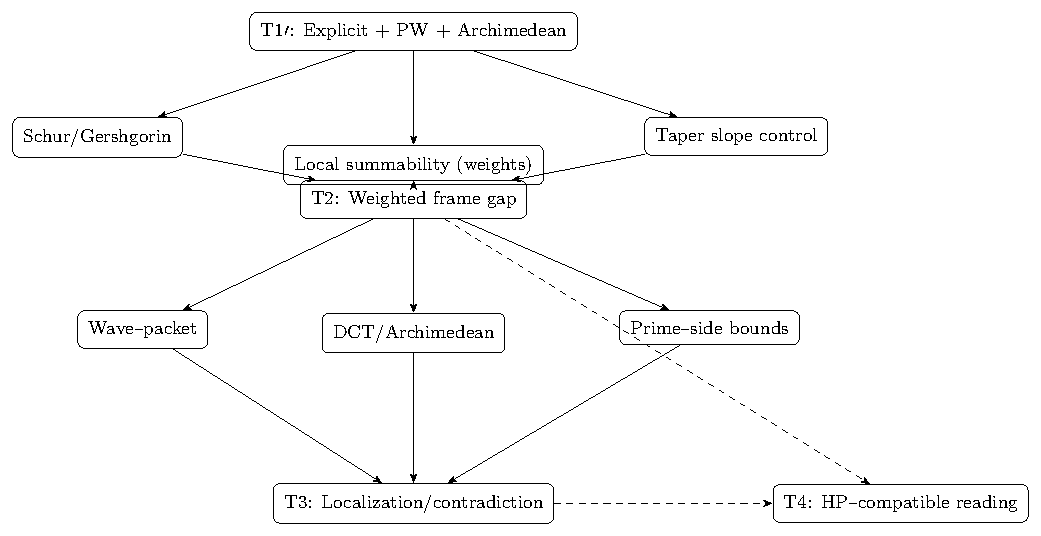
\includegraphics[width=.92\linewidth]{explication-grand-format/latex/graphe_dependances_standalone.pdf}
\end{frame}
\end{document}
